\chapter{The CMS Experiment at the LHC}
\label{chapter:three}
\section{The Large Hadron Collider}

The Large Hadron Collider (LHC) is the world’s largest and most powerful particle accelerator. Inside the accelerator, two highly energetic proton beams collide up to a center-of-mass energy of 14 TeV. The LHC is constructed inside a 27 km tunnel, 100 m under the ground, located partly in Switzerland and France.

At the LHC two energetic proton beams travel in opposite directions in separate beam pipes. The proton beams travel in bunches separated by 25 ns in time. The beams travel at relativistic speeds and collide at four major interaction points at the LHC. The LHC has four main detector experiments at each interaction point: ALICE (A Large Ion Collider Experiment), ATLAS (A Toroidal LHC Apparatus), CMS (Compact Muon Solenoid), and LHCb (Large Hadron Collider beauty). ATLAS and CMS are general purpose-detectors with broad physics objectives ranging from studying the Standard Model to searching Beyond Standard Model (BSM) physics such as Dark Matter. While ALICE and LHCb are more physics dedicated detectors, ALICE and LHCb are dedicated to heavy-ion physics and studying b-quark physics respectively.

%\begin{quotation}
%    \noindent Here is a block quotation---a passage from a text you found insightful and wanted to share with others. Maybe it is from a %journal article, website, or book. Irrespective, it should support the argument being made.\footnote{A citation for the quoted material.}
%\end{quotation}

%Check appendix \ref{appendix: chapter3}

%Maybe a sentence or two that bring the argument and evidence together.\citep{dos_santos_2020}



\section{The Compact Muon Solenoid Experiment}
\subsection{Introduction}
The Compact Muon Solenoid (CMS) is a general purpose detector located in eastern France at the Large Hadron Collider (LHC) tunnel 100 m underground. It is a general purpose detector because of its broad physics searches ranging from studying the Standard Model (SM) to searching for particles that could potentially make Dark Matter (DM). CMS is a cylindrical shaped detector with 21 m in length and 15 m in cross-sectional diameter. The three main characteristics of the CMS experiment are its compactness, accurate detection of Muon particles in the muon system and its magnetic solenoid. The superconducting magnetic solenoid at the core of the CMS detector produces a continuous magnetic field of 3.8 T which is of the order of O(5) of Earth's magnetic field (0.25 - 0.65 gaus). Such large magnetic field is required for a precise measurement of the momentum of high-energy charged particles. All CMS detector subsystems are enclosed by the magnetic solenoid, the muon system, on the other hand, is on the outside. Muons are the particles that are directly detected by the CMS, with a special property that they neither stop nor decay within the boundaries of the detector. They undergo very little energy loss and thus act as a powerful medium to study high-energy process in the presence of high background.
The CMS detector is cylindrical shaped with an onion like structure, having several concentric layers of subsystems. These subsystems help prepare "photographic images" of each collision event by determining the properties of the particles in the collision. CMS has the following basic subsystems ordered from innermost to outermost:

\begin{enumerate}
    \item Silicon Tracking Detector
    \item Electromagnetic Calorimeter
    \item Hadronic Calorimeter
    \item Superconducting Solenoid Magnet
    \item Muon System
    
    
\end{enumerate}
The CMS detector can detect 5 general categories of particles as shown in the figure below:
 \begin{enumerate}
    \item Electrons
    \item Photons
    \item Charged Hadrons
    \item Neutral Hadrons
    \item Muons
\end{enumerate}

\begin{figure} [tpb]
\centering
         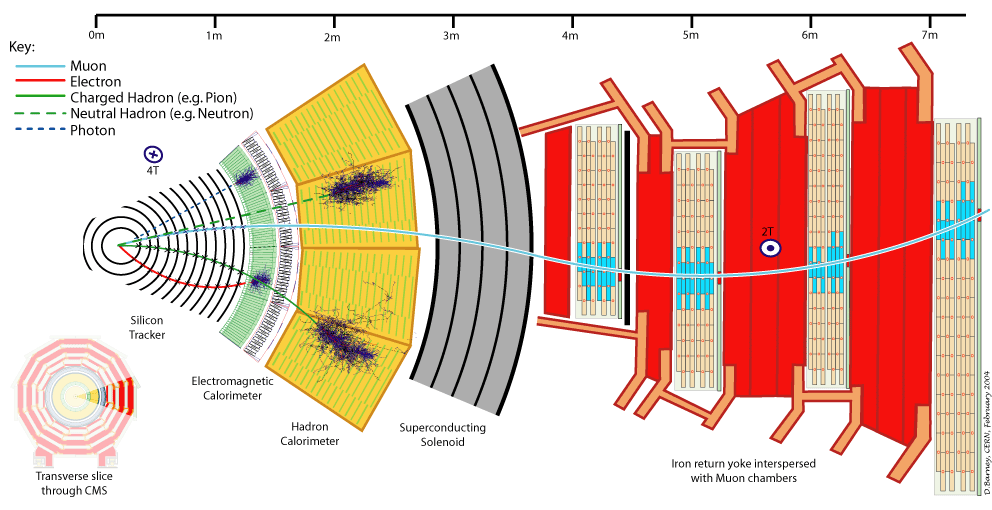
\includegraphics[width=0.9\textwidth,clip=]{thesis_template_cua/Figures/CMS_LHC_chapter/CMSSlice.png}
         \vspace*{10mm}
         \caption[#CMS Slice]{This Figure shows the cross-sectional slice of the CMS detector. Here we have shown the different sub-systems of CMS, trajectories and energy deposits of the 5 general categories of particles detected by CMS by one or more of its sub-systems}
         \label{cms:slice}
\end{figure}
%More ideas that really make this a great paper. Maybe a footnote or two.\footnote{Some peripheral thoughts that belong in a note.}
\subsection{Coordinate System}
The definition of a coordinate system is very crucial in quantifying the position of a particle inside CMS with respect to its center. The coordinate system at CMS is defined as follows and illustrated in Figure \Fig~\ref{cms:coordinate} -- the origin is defined as the nominal pp collision point,  the  $x$-axis points inwards towards the center of the LHC ring, the $y$-axis points upwards perpendicular to the $x$-axis and the $z$-axis points in the counter-clockwise beam direction. However, in hadron collider physics a more traditional coordinate, pseudo-rapidity $\eta$ is used, defined as

\begin{equation}
  \eta = -\ln\tan\left(\frac{\theta}{2}\right)
  \label{eq:eta}
\end{equation}

\begin{figure} [tpb]
\centering
         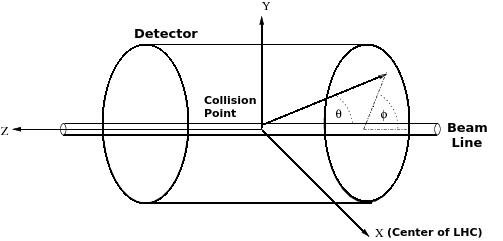
\includegraphics[width=0.9\textwidth,clip=]{thesis_template_cua/Figures/CMS_LHC_chapter/coord.png}
         \vspace*{10mm}
         \caption[#CMS Coordinate System]{This Figure shows the coordinate system used by the CMS detector adapted from ~\cite{Perez:coordinate}, illustrating the $x$-axis, $y$-axis, $z$-axis, radial angle $\theta$ (measured wrt to the $z$-axis and the azimuthal angle $\phi$ (measured in $x$-$y$ plane from the $x$-axis).}
         \label{cms:coordinate}
\end{figure}

For a particle of three-momentum $\textbf{p}$ with $z$-component $p_z$, pseudorapidity can be written as
\begin{equation}
  \eta = \frac12\ln\left(\frac{|\textbf{p}|+p_z}{|\textbf{p}|-p_z}\right)
  \label{eq:eta_p}
\end{equation}
In the limit of relativistic particles (high velocity and low mass limit), the pseudo-rapidity approximates the rapidity y given by
\begin{equation}
  y = \frac12\ln\left(\frac{E+p_z}{E-p_z}\right),
  \label{eq:rap}
\end{equation}
The rapidity is invariant under Lorentz boost transformations and is only dependent on the polar angle $\theta$ and not on the energy of the particle. From Figure \Fig~\ref{cms:rapidity}, we see that higher values of $\eta$ correspond to low values of $\theta$, this region is also referred as "forward" or high $\eta$ regions. In Figure \Fig~\ref{cms:rapidity}, we observe two regions which cover approximately  $|\eta| < 1.2$ and $1.2 <|\eta|  < 3$, these regions are known as the barrel and the endcap respectively.

\begin{figure} [tpb]
\centering
         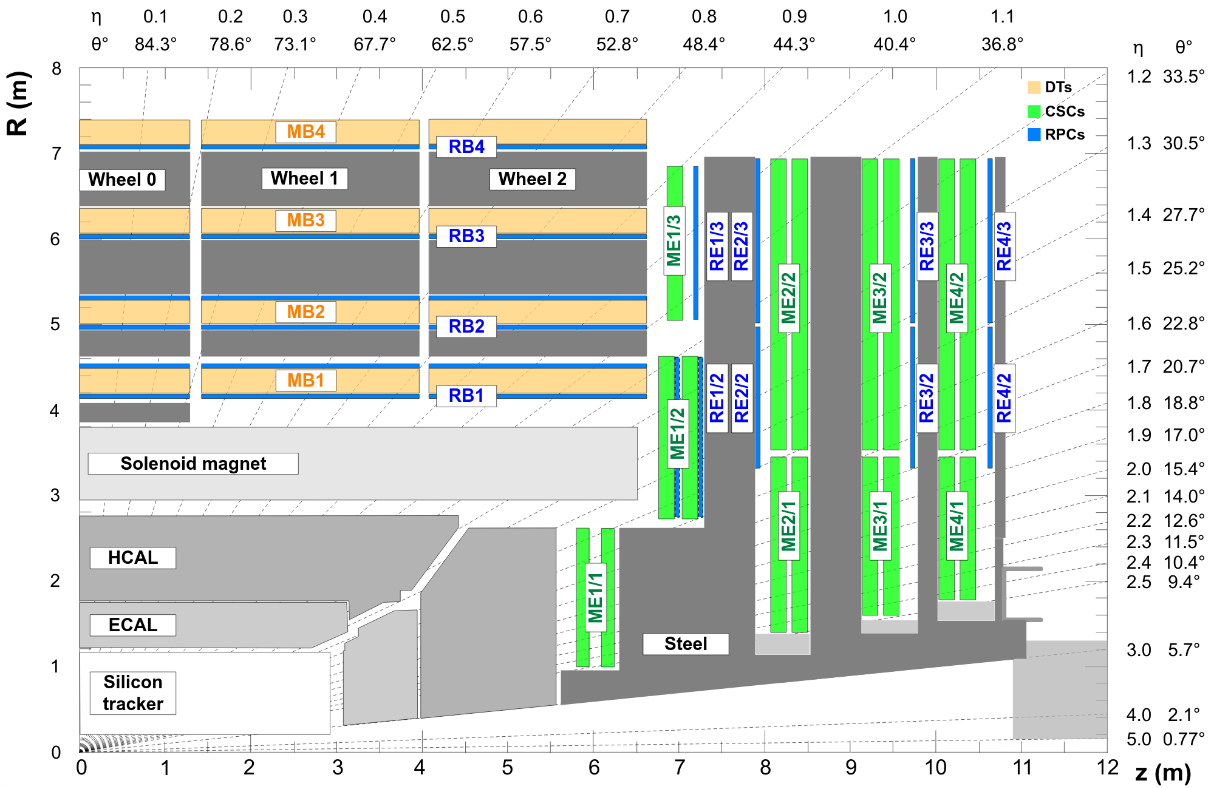
\includegraphics[width=0.9\textwidth,clip=]{thesis_template_cua/Figures/CMS_LHC_chapter/rapidity.png}
         \vspace*{10mm}
         \caption[#CMS Rapidity distribution]{This Figure shows one quadrant of CMS in the $r-z$ plane adapted from \cite{lee:rapidity}, illustrating the positions of subsystems in barrel and endcap regions}
         \label{cms:rapidity}
\end{figure}


\subsection{Silicon Tracking Detector}

\subsection{Electromagnetic Calorimeter}

\subsection{Hadronic Calorimeter}

\subsection{Solenoid Magnet}

\subsection{Muon System}

\subsubsection{DT}

\subsubsection{RPC}

\subsubsection{CSC}

\subsection{Trigger System}
